\documentclass{article}

\usepackage[colorlinks, urlcolor=blue, linkcolor=red, citecolor=green]{hyperref}
\usepackage{fancyhdr} %设置页眉和页脚的
\usepackage{extramarks} %设置continue那玩意的
\usepackage{amsmath}
\usepackage{amsthm}
\usepackage{amsfonts}
\usepackage{tikz} %画线的
\usepackage[plain]{algorithm}
\usepackage{algpseudocode}
\usepackage{enumerate}

\usetikzlibrary{automata,positioning}

%表
\usepackage{booktabs}
\usepackage{multirow}
\usepackage{array}
\usepackage{caption}
\DeclareCaptionFont{heiti}{\heiti} %还可以定义其他的
\captionsetup{labelsep=space, font={small, bf}, skip=2pt} %space可以改成quad

%图
%*****************图片及其相关设置***************************
\usepackage{graphicx}
\graphicspath{{tupian/}}
\usepackage{subfigure}

%*****************代码相关设置***************************
\usepackage{pythonhighlight}
%
% Basic Document Settings
%

\topmargin=-0.45in
\evensidemargin=0in
\oddsidemargin=0in
\textwidth=6.5in
\textheight=9.0in
\headsep=0.25in

\linespread{1.1}

\pagestyle{fancy}
\lhead{\hmwkAuthorName}
\chead{\hmwkClass: \hmwkTitle}
\rhead{\firstxmark}
\lfoot{\lastxmark}
\cfoot{\thepage}

\renewcommand\headrulewidth{0.4pt}
\renewcommand\footrulewidth{0.4pt}

\setlength\parindent{0pt}

%
% Create Problem Sections
%

\newcommand{\enterProblemHeader}[1]{
    \nobreak\extramarks{}{Problem \arabic{#1} continued on next page\ldots}\nobreak{}
    \nobreak\extramarks{Problem \arabic{#1} (continued)}{Problem \arabic{#1} continued on next page\ldots}\nobreak{}
}

\newcommand{\exitProblemHeader}[1]{
    \nobreak\extramarks{Problem \arabic{#1} (continued)}{Problem \arabic{#1} continued on next page\ldots}\nobreak{}
    \stepcounter{#1}
    \nobreak\extramarks{Problem \arabic{#1}}{}\nobreak{}
}

\setcounter{secnumdepth}{0}
\newcounter{partCounter}
\newcounter{homeworkProblemCounter}
\setcounter{homeworkProblemCounter}{1}
\nobreak\extramarks{Problem \arabic{homeworkProblemCounter}}{}\nobreak{}

\newenvironment{homeworkProblem}{
    \section{Problem \arabic{homeworkProblemCounter}}
    \setcounter{partCounter}{1}
    \enterProblemHeader{homeworkProblemCounter}
}{
    \exitProblemHeader{homeworkProblemCounter}
}

%
% Homework Details
%   - Title
%   - Due date
%   - Class
%   - Section/Time
%   - Instructor
%   - Author
%

\newcommand{\hmwkTitle}{Homework\ \#3}
\newcommand{\hmwkDueDate}{April 28, 2021}
\newcommand{\hmwkClass}{Deep Learning}
\newcommand{\hmwkClassTime}{}
\newcommand{\hmwkClassInstructor}{Professor Zhen Li}
\newcommand{\hmwkAuthorName}{Haoyu Kang}
\newcommand{\hmwkAuthorSchool}{School of Data Science}
\newcommand{\hmwkAuthorNumber}{Sno.220041025}
%
% Title Page
%

\title{
    \vspace{2in}
    \textmd{\textbf{\hmwkClass:\ \hmwkTitle}}\\
    \normalsize\vspace{0.1in}\small{Due\ on\ \hmwkDueDate}\\
	\vspace{0.1in}\large{\textit{\hmwkClassInstructor\ \hmwkClassTime}}\\
    \vspace{3in}
}

\author{\textbf{\hmwkAuthorName}\\\textbf{\hmwkAuthorNumber}}


\date{}

\renewcommand{\part}[1]{\textbf{\large Part \Alph{partCounter}}\stepcounter{partCounter}\\}

%
% Various Helper Commands
%

% Useful for algorithms
\newcommand{\alg}[1]{\textsc{\bfseries \footnotesize #1}}
\usepackage[algo2e,vlined,ruled]{algorithm2e}

% For derivatives
\newcommand{\deriv}[1]{\frac{\mathrm{d}}{\mathrm{d}x} (#1)}

% For partial derivatives
\newcommand{\pderiv}[2]{\frac{\partial}{\partial #1} (#2)}

% Integral dx
\newcommand{\dx}{\mathrm{d}x}

% Alias for the Solution section header
\newcommand{\solution}{\textbf{\large Solution}}

% Probability commands: Expectation, Variance, Covariance, Bias
\newcommand{\E}{\mathrm{E}}
\newcommand{\Var}{\mathrm{Var}}
\newcommand{\Cov}{\mathrm{Cov}}
\newcommand{\Bias}{\mathrm{Bias}}
\begin{document}

\maketitle
\thispagestyle{empty}

\newpage
\setcounter{page}{1}

\begin{homeworkProblem}

	\textbf{\large{Solution}}
	
	\vspace{4pt}
	\textbf{Subproblem (a)}
	
	\begin{equation}
		\label{eq1}
		\begin{split}
	[[L_tf]*w](x)=&\sum_{y \in Z^2}\sum_{k=1}^K[L_tf]_k(y)w_k(y-x)\\
	=&\sum_{y \in Z^2}\sum_{k=1}^Kf_k(y-t)w_k(y-x)\\
	=&\sum_{y \in Z^2}\sum_{k=1}^K f_k(y)w_k(y+t-x)\\
	=&\sum_{y \in Z^2}\sum_{k=1}^K f_k(y)w_k(y-(x-t)\\
	[[L_tf]*w](x)=&[f*w](x-t)\\
	=&\sum_{y \in Z^2}\sum_{k=1}^K f_k(y)w_k(y-(x-t)\\
        \end{split}
    \end{equation}
	
	\textbf{Subproblem (b)}
	
	\begin{equation}
		\label{eq4}
		\begin{split}
			[[L_Rf]*w](x)=&\sum_{y \in Z^2}\sum_{k=1}^K[L_Rf]_k(y)w_k(y-x)\\
	=&\sum_{y \in Z^2}\sum_{k=1}^Kf_k(R^{-1}y)w_k(y-x)\\
	=&\sum_{y \in Z^2}\sum_{k=1}^K f_k(y)w_k(Ry-x)\\
	=&\sum_{y \in Z^2}\sum_{k=1}^K f_k(y)w_k(R(y-R^{-1}x)\\
	=&\sum_{y \in Z^2}\sum_{k=1}^K f_k(y)([L_{R^{-1}}w]_k(y-R^{-1}x))\\
	L_R[f*[L_{R^{-1}}w]](x)=&[f*[L_{R^{-1}}w]](R^{-1}x)\\
	=&\sum_{y \in Z^2}\sum_{k=1}^K f_k(y)([L_{R^{-1}}w]_k(y-R^{-1}x))\\
		\end{split}
	\end{equation}	
	
	
	
	
	\textbf{Subproblem (c)}
	
	\begin{equation}
		\label{eq4}
		\begin{split}
			[[L_uf]*w](g)=&\sum_{h \in G}\sum_{k=1}^K[L_uf]_k(h)w_k(g^{-1}h)\\
	=&\sum_{h \in G}\sum_{k=1}^Kf_k(u^{-1}h)w_k(g^{-1}h)\\
	=&\sum_{h \in G}\sum_{k=1}^K f_k(h)w_k(g^{-1}uh)\\
	=&\sum_{h \in G}\sum_{k=1}^K f_k(h)w_k((u^{-1}g)^{-1}h)\\
	=&[f*w](u^{-1}g)=[L_u[f*w]](g)\\
		\end{split}
	\end{equation}
	
	
\end{homeworkProblem}

\begin{homeworkProblem}
	\vspace{4pt}
	\textbf{\large{Solution}}

	\vspace{4pt}
	\begin{equation}
		\begin{split}
			{\partial L\over \partial W_{hz}}=&\sum_t{\partial L_t\over \partial W_{hz}}=\sum_t{\partial L_t\over \partial z_t}{\partial z_t\over \partial net_t}{\partial net_t\over \partial w_{hz}}\\
			=& \sum_{t} \begin{bmatrix} &0&  \\ &0& \\ &\vdots& \\ &-1 \over{Z_k}&\\ &\vdots& \\ &0 \end{bmatrix}^{\top} \cdot 
			\begin{bmatrix} {\partial Z_{t,1} \over {\partial {Net_{t,1}}}} &\cdots& {\partial Z_{t,1} \over {\partial {Net_{t,c}}}}\\ &\vdots&\\ {\partial Z_{t,c} \over {\partial {Net_{t,1}}}} &\cdots& {\partial Z_{t,c} \over {\partial {Net_{t,c}}}}\end{bmatrix}
			\cdot \begin{bmatrix} h_{t,1} & h_{t,2} &\cdots& h_{t,c}\end{bmatrix}\\
			=& \sum_{t} \left\{\begin{bmatrix} 0&0 &\cdots& {-1 \over{Z_k}} &\cdots& 0 \end{bmatrix} \cdot 
			\begin{bmatrix} {Z_{t,1}-Z_{t,1}^2 }&{-Z_{t,1}Z_{t,2}} &\cdots& {-Z_{t,1}Z_{t,c}}\\ &\vdots&\\ 
				{-Z_{t,1}Z_{t,c}}&{-Z_{t,c}Z_{t,2}} &\cdots &{Z_{t,c}-Z_{t,c}^2 }\end{bmatrix}\right\}^{\top}
			\cdot \begin{bmatrix} h_{t,1} & h_{t,2} &\cdots& h_{t,c}\end{bmatrix}\\
			=& \sum_{t}(\boldsymbol{Z_{t}}-\boldsymbol{y_t})^{\top}h_t
		\end{split}
	\end{equation}	

	\vspace{4pt}
	\begin{equation}
		\begin{split}
			{\partial L\over \partial W_{hh}}=&\sum_t{\partial L_t\over \partial W_{hh}}=\sum_t({\partial L_t\over \partial z_t}{\partial z_t\over \partial net_t}{\partial net_t\over \partial h_{t}}+{\partial L_{t+1}\over \partial z_{t+1}}{\partial z_{t+1}\over \partial net_t}{\partial net_{t+1}\over \partial h_{t+1}}{\partial net_{t+1}\over \partial h_{t}}){\partial h_t \over \partial hidden_t }{\partial hidden_t \over \partial W_{hh} }\\
			=& \sum_{t} \begin{bmatrix} &0&  \\ &0& \\ &\vdots& \\ &-1 \over{Z_k}&\\ &\vdots& \\ &0 \end{bmatrix}^{\top} \cdot 
			\begin{bmatrix} {\partial Z_{t,1} \over {\partial {Net_{t,1}}}} &\cdots& {\partial Z_{t,1} \over {\partial {Net_{t,c}}}}\\ &\vdots&\\ {\partial Z_{t,c} \over {\partial {Net_{t,1}}}} &\cdots& {\partial Z_{t,c} \over {\partial {Net_{t,c}}}}\end{bmatrix}
			\cdot \begin{bmatrix} W_{hz,1} & W_{hz,2} &\cdots& W_{hz,c}\end{bmatrix}+\\
			& \begin{bmatrix} &0&  \\ &0& \\ &\vdots& \\ &-1 \over{Z_k}&\\ &\vdots& \\ &0 \end{bmatrix}^{\top} \cdot 
			\begin{bmatrix} {\partial Z_{t+1,1} \over {\partial {Net_{t+1,1}}}} &\cdots& {\partial Z_{t+1,1} \over {\partial {Net_{t+1,c}}}}\\ &\vdots&\\ {\partial Z_{t+1,c} \over {\partial {Net_{t+1,1}}}} &\cdots& {\partial Z_{t+1,c} \over {\partial {Net_{t+1,c}}}}\end{bmatrix}
			\cdot \begin{bmatrix} W_{hz,1} & W_{hz,2} &\cdots& W_{hz,c}\end{bmatrix}\cdot W_{hh} \cdot tanh'(hidden_t)\cdot h_{t-1}\\
			=&\sum_t [(Z_t-y_t)^T W_{hz}+(Z_{t+1}-y_{t+1})^T W_{hz}^T W_{hh}]tanh'(hidden_t)\cdot h_{t-1}
		\end{split}
	\end{equation}
\vspace{4pt}


		
\end{homeworkProblem}

\begin{homeworkProblem}

\textbf{\large{Solution}}
	
\vspace{4pt}
\textbf{Subproblem (a)}

\vspace{4pt}
	
$\circ$ Given $(s,a,r,s')$, we use the update equation:
\begin{equation}
	\begin{split}
	\label{eq7}
	Q(s,a)\leftarrow Q(s,a)+\alpha(r+\gamma \quad max_{a'\in \left\{-1,1\right\}} \quad Q(s',a')-Q(s,a))
	\end{split}			
\end{equation}

$\circ$ Using the equation with $\alpha={1\over 2}, \gamma={1\over 3}$, we have:
\begin{equation}
	\begin{split}
		Q(3,-1)\leftarrow& 0+{1\over 2}(-1+{1\over 3}max_{a'}Q(2,a'))=-{1\over 2}\\
		Q(2,-1)\leftarrow& 0+{1\over 2}(-1+{1\over 3}max_{a'}Q(3,a'))=-{1\over 2}\\
		Q(3,1)\leftarrow& 0+{1\over 2}(-1+{1\over 3}max_{a'}Q(4,a'))=-{1\over 2}\\
	\end{split}
\end{equation}

\textbf{Subproblem (b)}

\vspace{4pt}

$\circ$ We have $\nabla_wJ(w)$ as follow:
\begin{equation}
	\begin{split}
	\label{eq7}
	\nabla_w J(w)=&-2(r+\gamma max_{a'}\hat{q}(s',a';w^-)-\hat{q}(s,a;w))\nabla_w \hat{q}(s,a;w)\\
=&-2(r+{1\over 3}max_{a'}(w^-)^T\begin{bmatrix}
	s'\\a'\\1\end{bmatrix}-w^T\begin{bmatrix}s\\a\\1\end{bmatrix})\begin{bmatrix}
		s\\a\\1
	\end{bmatrix}
	\end{split}			
\end{equation}
\vspace{4pt}

$\circ$ using this, the parameter update with a single sample $(s,a,r,s') $ is:

\begin{equation}
	\begin{split}
		w'\rightarrow& w-\alpha \nabla_wJ(w)\\
		=&w+{1\over2}(r+{1\over 3}max(w^-)^T\begin{bmatrix}
			s'\\a'\\1
		\end{bmatrix}-w^T\begin{bmatrix}
			s\\a\\1
		\end{bmatrix})\begin{bmatrix}
			s\\a\\1
		\end{bmatrix}
	\end{split}
\end{equation}

$\circ$ Usiing the sample $(2,-1,-1,1)$ and the particular values of $w$ and $w^-$ yields:
\begin{equation}
	\begin{split}
		w'\rightarrow& \begin{bmatrix}
			-1\\1\\1 
		\end{bmatrix}+{1\over 2}(-1+{1\over3} max_{a'}\begin{bmatrix}
			1\\-1\\-2
		\end{bmatrix}^T\begin{bmatrix}
			1\\a'\\1
		\end{bmatrix}-\begin{bmatrix}
			-1\\1\\1
		\end{bmatrix}^T\begin{bmatrix}
			2\\-1\\1
		\end{bmatrix})\begin{bmatrix}
			2\\-1\\1
		\end{bmatrix}\\
		=&\begin{bmatrix}
			-1\\1\\1 
		\end{bmatrix}+{1\over 2}(-1+{1\over3} max_{a'}(1-a'-2)-(-2-1+1))\begin{bmatrix}
			2\\-1\\1\end{bmatrix}\\
		=&\begin{bmatrix}
			-1\\1\\1
		\end{bmatrix}+{1\over 2}\begin{bmatrix}
			2\\-1\\1
		\end{bmatrix}\\
		=&\begin{bmatrix}
			0\\ 1/2 \\3/2
		\end{bmatrix}
	\end{split}
\end{equation}


	
\end{homeworkProblem}
\begin{homeworkProblem}

	\textbf{\large{Solution}}
	
	\vspace{4pt}

	The picture of plotting of training curve and test accuracy under 4 subprobelms is shown as follow:
	\begin{center}
		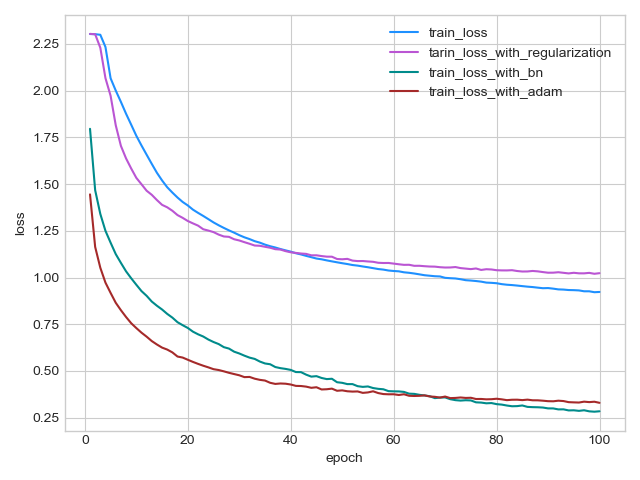
\includegraphics[width=12cm,height=8cm]{1.png}
	 \end{center}
	 \begin{center}
		Fig 1: Loss vs Epoch
	 \end{center}

	 \begin{center}
		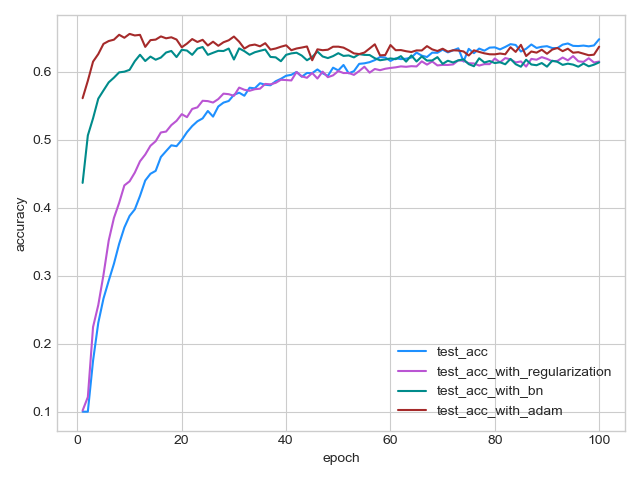
\includegraphics[width=12cm,height=8cm]{2.png}
	 \end{center}
	 \begin{center}
		Fig 2: Accuracy vs Epoch
	 \end{center}
	
\textbf{Subproblem (a)}
\vspace{4pt}

After using softmax loss and regularization, we find that trian loss varies a little compared with original setting. However the test accuracy 
increase at the early time since it overcomes the overfitting that is brought in original setting. The visulization of first layer filter is as follow:
\begin{center}
	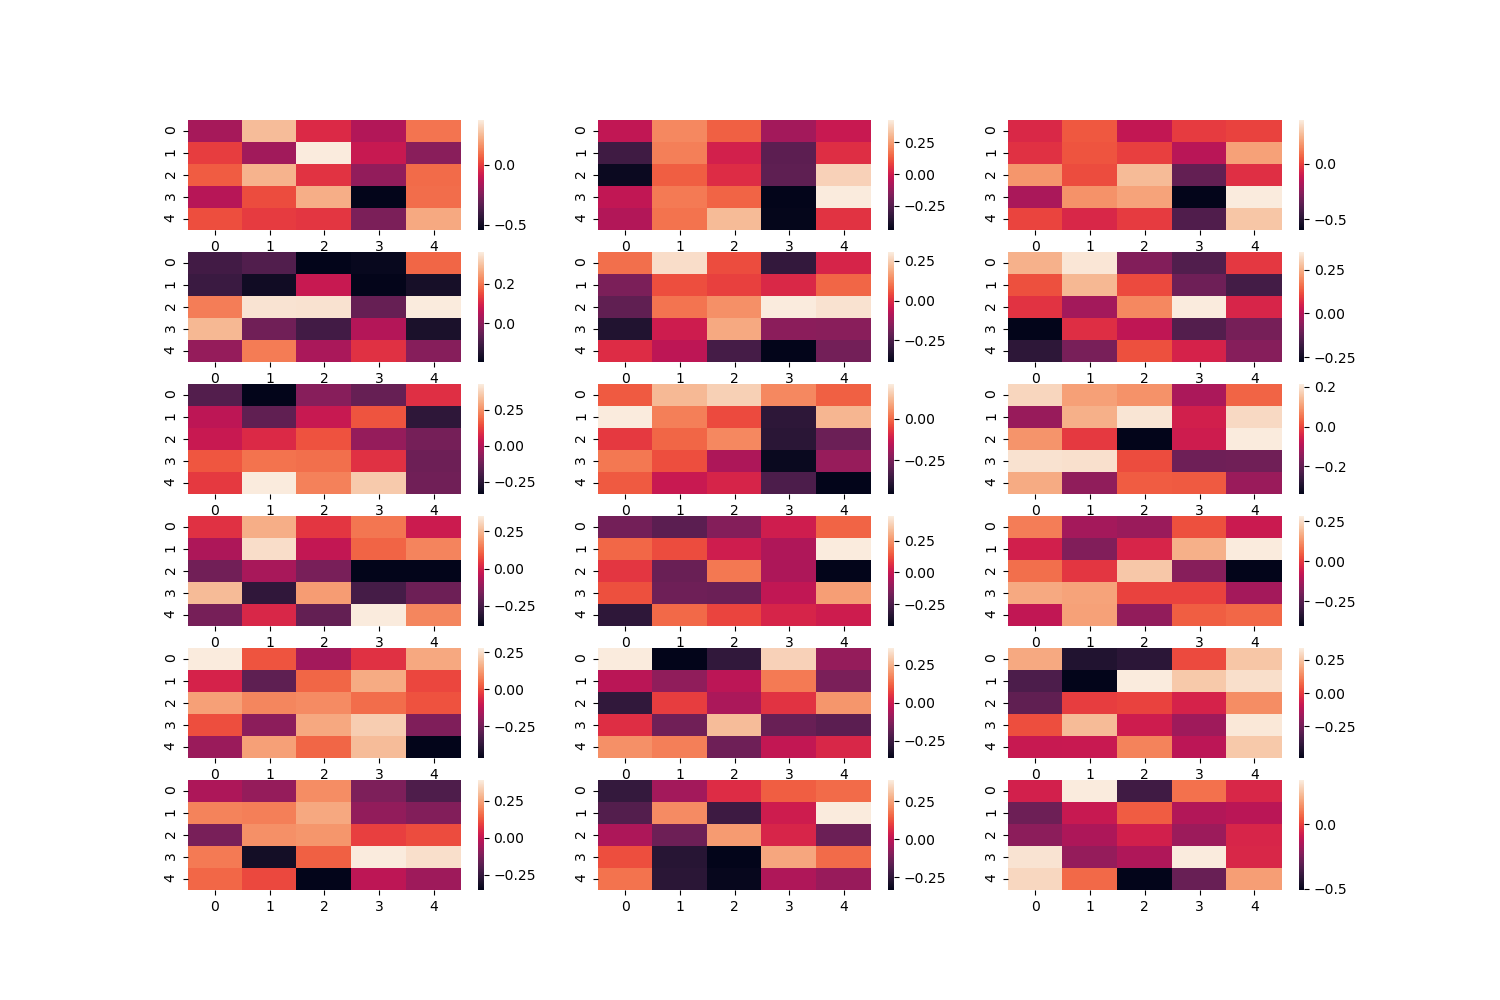
\includegraphics[width=15cm,height=10cm]{heatmap.png}
 \end{center}
 \begin{center}
	Fig 3: The filters learned in the first convolutional layer
 \end{center}

\textbf{Subproblem (b)}
\vspace{4pt}

$\circ$ We prove $Var[y_l]=n_l Var[w_l]E[x_l^2]$ as follow

\begin{equation}
	\begin{split}
		Var[y_l]=&Var[W_{l,i}\cdot x_l]\\
=&n_l\cdot Var[w_l\cdot x_l]\\
=&n_l\cdot(E[(w_l\cdot x_l)^2]-(E[w_l\cdot x_l])^2)\\
=&n_l\cdot(E[(w_l\cdot x_l)^2]-(E[w_l]\cdot E[x_l])^2)\\
=& n_l \cdot E[(w_l \cdot x_l)^2]\\
=& n_l \cdot E[w_l^2]\cdot E[x_l^2]\\
=& n_l \cdot Var[w_l]\cdot E[x^2_l]
	\end{split}
\end{equation}

$\circ$

\begin{equation}
	\begin{split}
		P(x)=&\begin{cases}
			0 \qquad x<0\\
			{1\over 2} \qquad x=0\\
			Q(x)  \qquad x>0\\
		\end{cases}\\ \\
	p(x)=&q(x) \qquad (x>0)
	\end{split}
\end{equation}

Then, we can have
\begin{equation}
	\begin{split}
		E[x_l^2]=&\int_{-\infty}^{\infty} x_l^2\cdot p(x_l) \,dx \\
		=&0^2\cdot {1\over2} + \int_{0}^{\infty} x_l^2\cdot p(x_l) \,dx\\
		=&\int_{0}^{\infty} x_l^2\cdot q(x_l)\,dx
	\end{split}
\end{equation}

We can also have
\begin{equation}
	\begin{split}
		{1\over 2}Var[y_l-1]=&{1\over 2}E(y^2_{l-1})\\
							=&{1\over 2}\int_{-\infty}^{\infty} y_{l-1}^2\cdot q(y) \,dy \\
							=&{1\over 2}\cdot 2\int_{0}^{\infty} y_{l-1}^2\cdot q(y) \,dy \\
							=&\int_{0}^{\infty} y_{l-1}^2\cdot q(y) \,dy \\
	\end{split}
\end{equation}

\vspace{4pt}
\textbf{Subproblem (c)}
\vspace{4pt}

From the figure, we see that training loss decrease quickly in the early stage after we add batch nomalization layer.
 That is becasue BN avoid covariance shift and gradient explosion and disappearance, which  accelerate convergece of training loss. In the meanwhile, test accuracy also 
 rise in the begining.

 \vspace{4pt}
\textbf{Subproblem (d)}
\vspace{4pt}

In this part, I use Adam optimizer to investigate if it can solve current trouble. Since adam utilize momentum and adaptive size to upgrade in rach iteration, so it has great
speed to decrease that we can see in the figure. At the begining of first 20 epochs, the model with Adam optimizer perform better on both training and testing.


\end{homeworkProblem}



\end{document}
